\begin{figure}[t]
  \begin{subfigure}[b]{0.35\textwidth}
    
\includegraphics[width=\textwidth]{./img/raw/lc-frame-example/ts/si_frame_250.png}
    \caption{Tiled Shading frame $250$.}
    \vspace{2pt}
    \label{fig:cs-test-frames-example:zc:250ts}
  \end{subfigure}\quad %
  \begin{subfigure}[b]{0.35\textwidth}
    
\includegraphics[width=\textwidth]{./img/raw/lc-frame-example/cs/si_frame_250.png}
    \caption{Lichtberekeningen frame $250$.}
    \vspace{2pt}
    \label{fig:cs-test-frames-example:sa:250cs}
  \end{subfigure}\\
  \begin{subfigure}[b]{0.35\textwidth}
    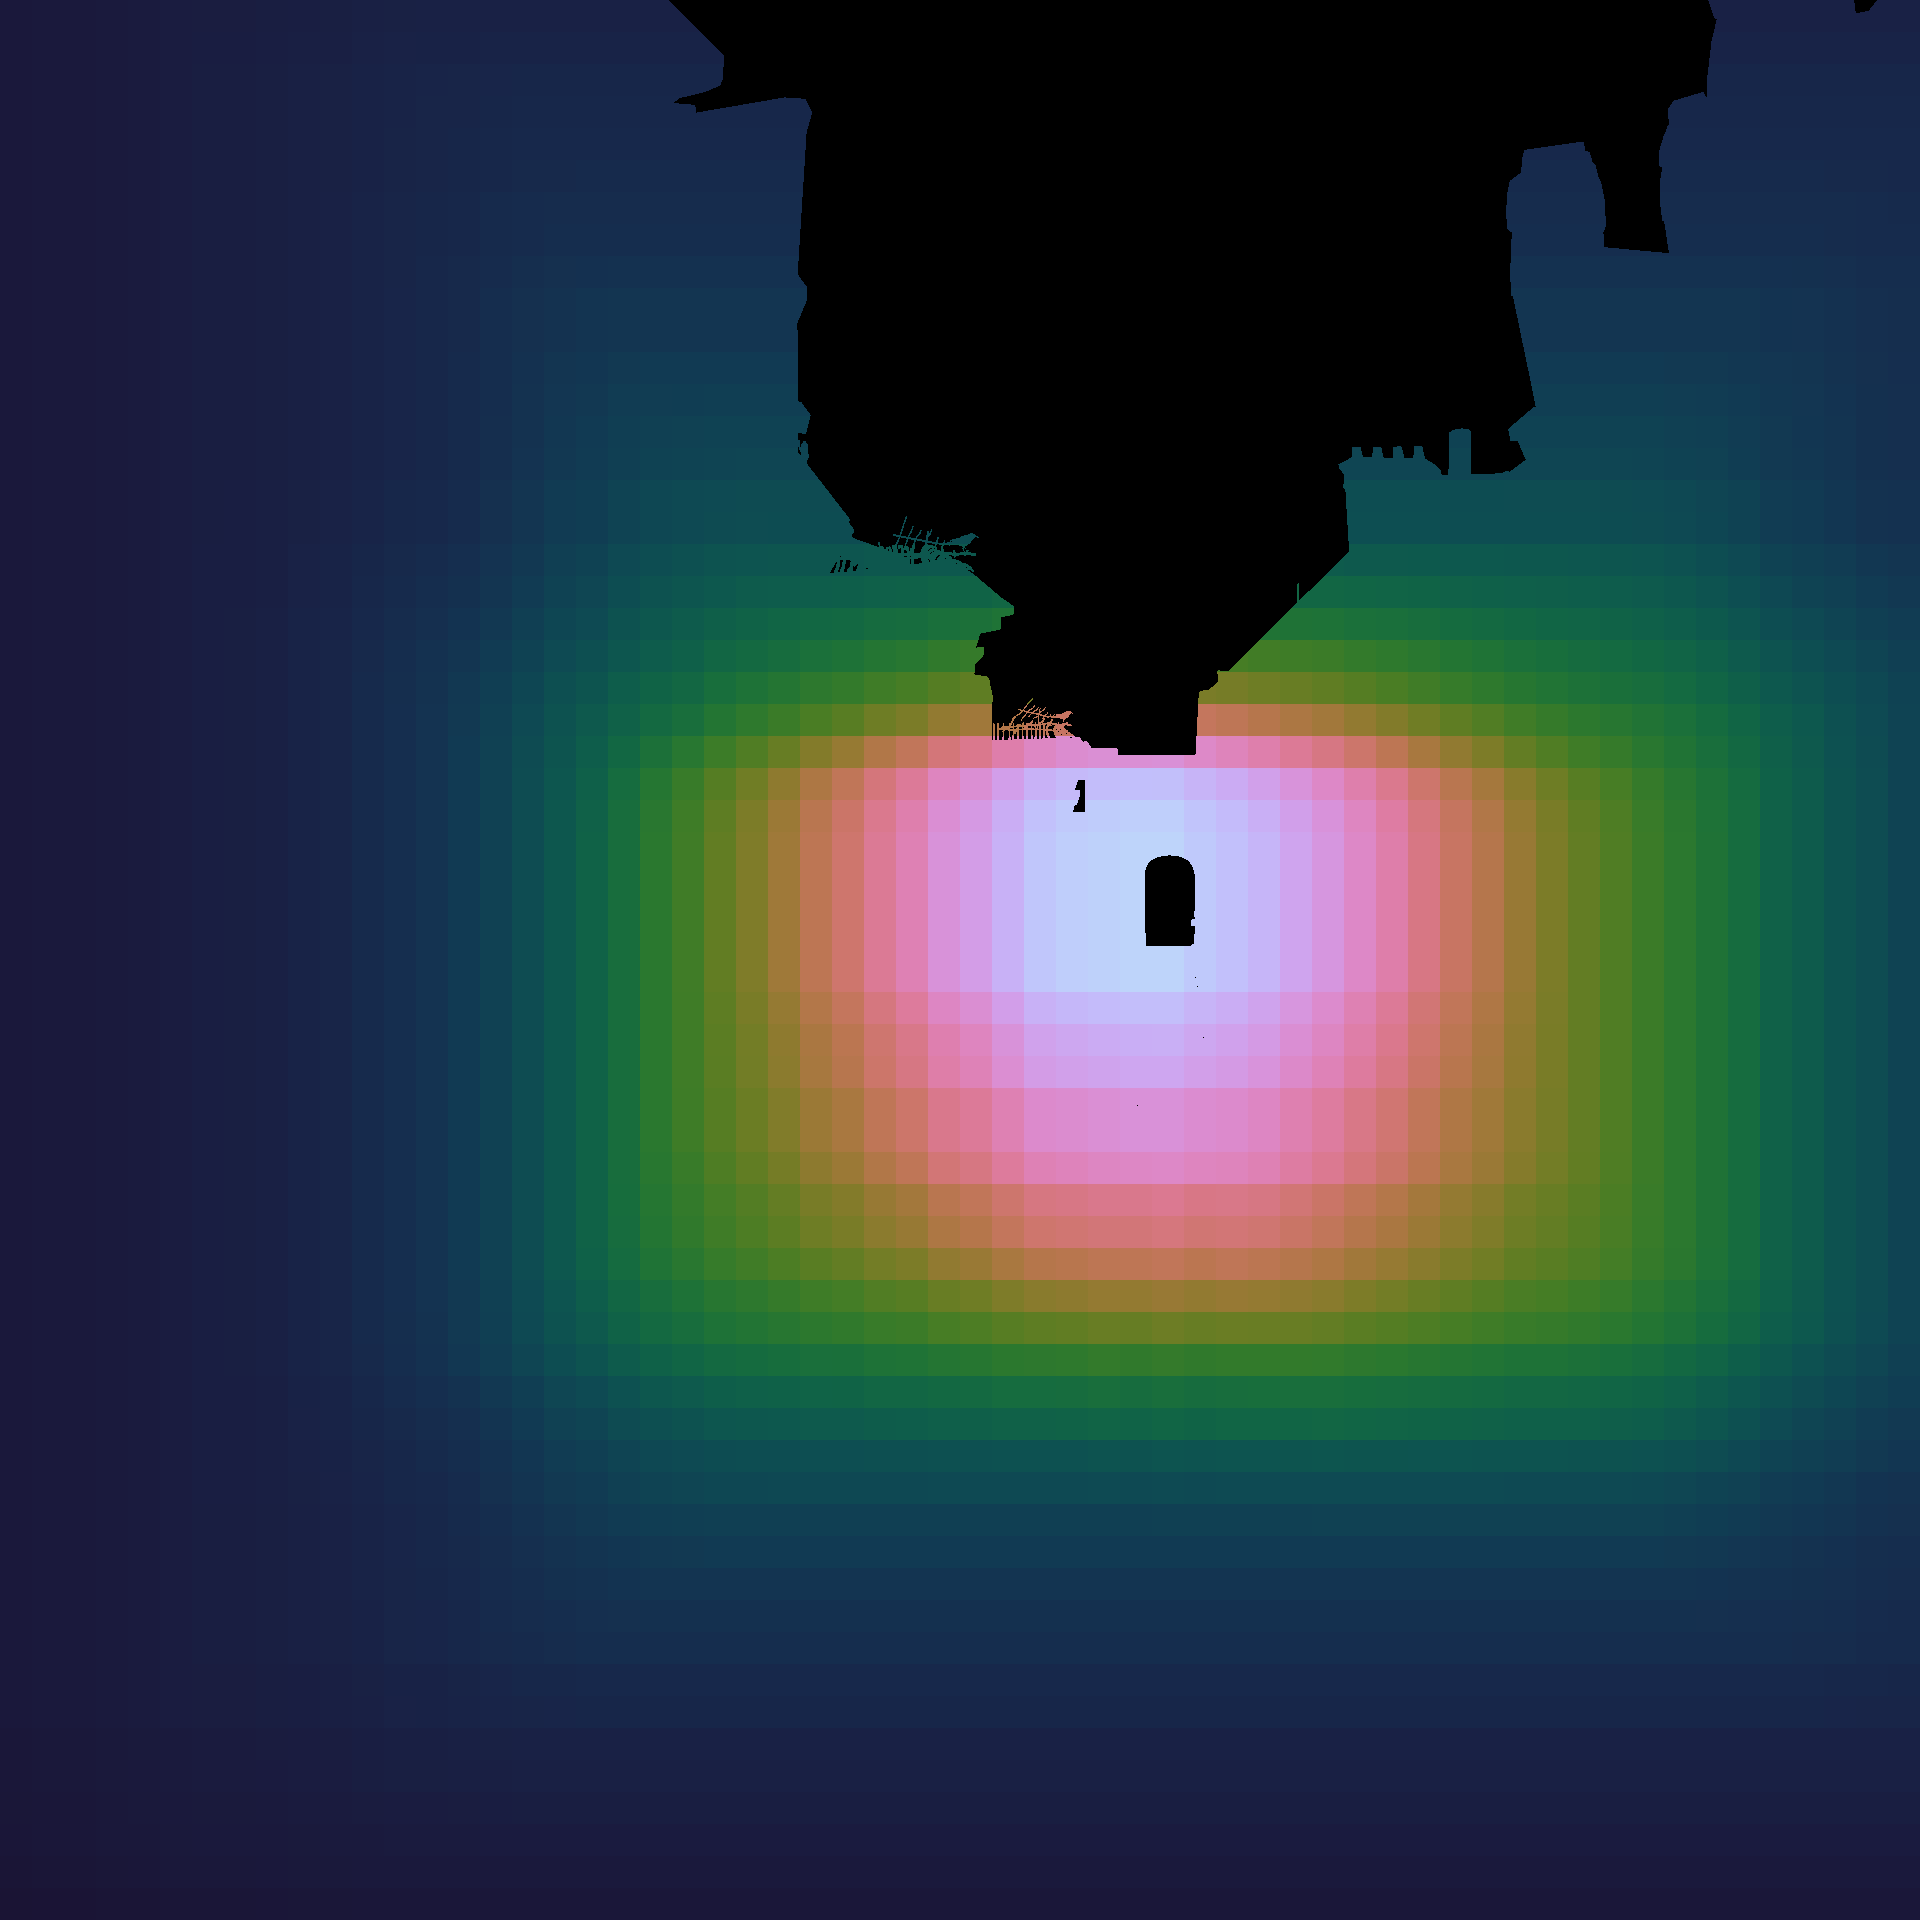
\includegraphics[width=\textwidth]{./img/raw/lc-frame-example/ts/pa_frame_126.png}
    \caption{Tiled Shading frame $126$.}
    \vspace{2pt}
    \label{fig:cs-test-frames-example:pa:126ts}
  \end{subfigure}\quad %
  \begin{subfigure}[b]{0.35\textwidth}
    
\includegraphics[width=\textwidth]{./img/raw/lc-frame-example/cs/pa_frame_126.png}
    \caption{Lichtberekening frame $126$.}
    \vspace{2pt}
    \label{fig:cs-test-frames-example:pa:126cs}
  \end{subfigure}\\
  \begin{subfigure}[b]{0.35\textwidth}
    
\includegraphics[width=\textwidth]{./img/raw/lc-frame-example/ts/zc_frame_417.png}
    \caption{Tiled Shading frame $417$.}
    \label{fig:cs-test-frames-example:zc:417ts}
  \end{subfigure}\quad %
  \begin{subfigure}[b]{0.35\textwidth}
    
\includegraphics[width=\textwidth]{./img/raw/lc-frame-example/cs/zc_frame_417.png}
    \caption{Lichtberekening frame $417$.}
    \label{fig:cs-test-frames-example:zc417cs}
  \end{subfigure}
  \caption{ Renders en hittekaarten van de verschillende scenes voor Tiled Shading.}
  \label{fig:cs-test-frames-example:zc}
\end{figure}

